
\documentclass[12pt,journal,compsoc]{IEEEtran}

\usepackage{graphicx}
\usepackage[table]{xcolor}
\setlength{\textfloatsep}{10pt plus 1.0pt minus 2.0pt}
\setlength{\floatsep}{2.0pt plus 2.0pt minus 2.0pt}
\setlength{\intextsep}{1.0pt plus 2.0pt minus 2.0pt}

\begin{document}

\begin{titlepage}
	\begin{center}
	\vspace*{1cm}
	University of California, Santa Cruz
	\vfill
	\textbf{The Physics of Figure Skating Jumps}  \\
	A technical paper about the physics of the 3 figure skating jumps.
	\vfill
	
	%\includegraphics[scale=.25]{2.JPG}
	
	%\vfill

	Intended Audience: \\ People interested in figure skating and physics. 

	Style Guide: MLA
	\vspace{0.8cm} \\
	\textbf{Christy Yuen}  \\
	Technical Writing for Computer Science and Engineering - CSE185S  \\
	Professor Gerald Moulds \\
	December 12th, 2020
   \end{center}
\end{titlepage}

\title{The Physics of Figure Skating Jumps}
\author{Christy Yuen}
\date{\today}		% leaving the brackets empty omits the date
% To input the current date, you can type: \date{\today}

% The paper headers
\markboth{The Physics of Figure Skating Jumps}%
{Yuen \MakeLowercase{\textit{et al.}}: CSE185}

%\IEEEpubid{0000--0000/00\$00.00~\copyright~2007 IEEE}

\IEEEcompsoctitleabstractindextext{%
\begin{abstract}
%\boldmath
The abstract goes here.
\end{abstract}

\begin{IEEEkeywords}
Toe Pick, Toe Loop, Salchow, Loop, Flip, Lutz, Axel, and Angular Momentum.
\end{IEEEkeywords}}

\maketitle

%\centerline{ \includegraphics[scale=.25]{2.JPG}}

%Introduction --------------------------------------------------------------

\section{Introduction}

\IEEEPARstart{T}{here} are 6 common figure skating jumps for competition. They are the Toe Loop, Salchow, Loop, Flip, Lutz, and Axel. 
Here is a diagram and terms we will be using. 
\begin{figure}[h]
	\centering
	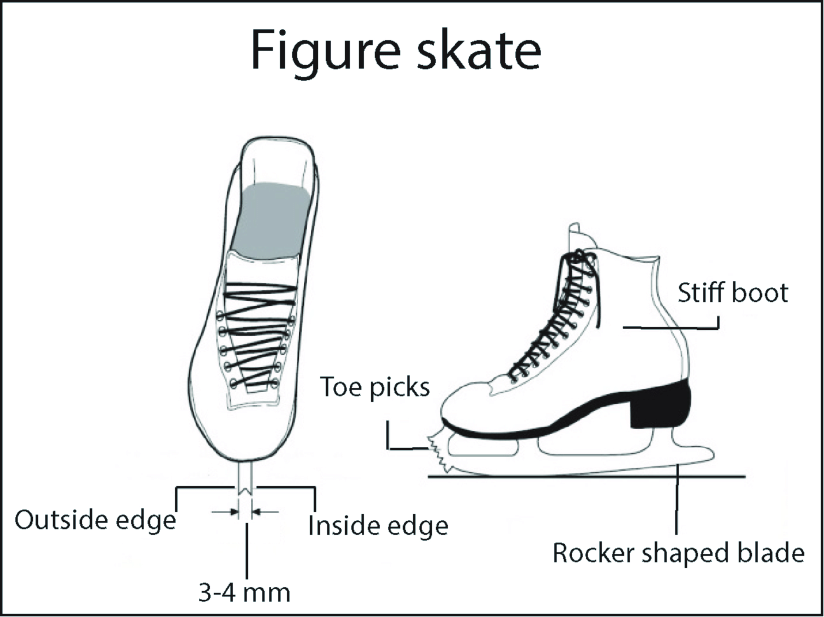
\includegraphics[scale=.25]{Skate_Diagram.PNG}
	\caption{Skate Diagram}
	\label{Fig:Skate_Diagram}
\end{figure}

A figure skaters' skate diagram. Here as shown, there is an inner edge and outer edge. This helps to understand where the skater is launching from and landing on. The Toe Pick helps in launching and landings too, and is located at the front of the skate. 
%Single Jumps --------------------------------------------------------------
\subsection{Scoring for Single Jumps}
\begin{center}
\rowcolors{2}{white}{gray!25}
  \begin{tabular}{|c|c|}
  \hline
  \multicolumn{2}{|c|}{Single Jump} \\
    %\rowcolor{gray!40}
    \hline
    \textbf{Jump (1 Rotation)} & \textbf{Base Value}\\
    \hline
    Toe Loop & 0.4\\
    \hline
    Salchow & 0.4\\
    \hline
    Loop & 0.5\\
    \hline
    Flip & 0.5\\
    \hline
    Lutz & 0.6\\
    \hline
    Axel & 1.1\\
    \hline
  \end{tabular}
\end{center}

%Quad Jumps --------------------------------------------------------------
\subsection{Scoring for Quad Jumps}
\begin{center}
\rowcolors{2}{white}{gray!25}
  \begin{tabular}{|c|c|}
  	\hline
	\multicolumn{2}{|c|}{Quad Jumps}  \\
	\hline
    \textbf{Jump (4 Rotation)} & \textbf{Base Value}\\
    \hline
    Quad Toe Loop & 10.3 \\
    \hline
    Quad Salchow & 10.5 \\
    \hline
    Quad Loop & 12.0 \\
    \hline
    Quad Flip & 12.3 \\
    \hline
    Quad Lutz & 13.6 \\
    \hline
    Quad Axel & 15.0 \\
    \hline
  \end{tabular}
\end{center}

%Toe Loop --------------------------------------------------------

\section{The Toe Loop Jump}
Invented by Bruce Mapes in the 1920s, the Toe Loop is one of the simplest jumps out of the six jumps. 

\subsection{The Toe Loop}
The Toe Loop starts with a forward approach on the inside edge of the skate's blade. Then, the skater "switches to a backward-facing orientation, kicking off with the backward outside edge and using a toe pick to add lift before landing on that same outside edge."

\subsection{The Physics of a Single Toe Loop}
The physics of a single Toe Loop is relatively simple. There is angular momentum acting on the skater as they launch and spin. There is vertical velocity as the skater moves from their jump to landing, and there is gravity acting on the skater as they land. The launch of a single jump isn't as hard as a triple or quad jump, as the height isn't much of a factor in the jump. But when the skater lands, on a single blade of their skate and on ice, that's when knowing what forces are acting on the skater determines if their landing is successful. For the Toe Loop, there is more angular momentum as the toe pick helps the skater create more spin to their jump. 

\subsection{The Physics of The Quad Toe Loop}
Using a study done by [NAME] called "Characteristics of triple and quadruple toe‐loops performed during the salt lake city 2002 winter olympics", this study will helps in terms of numbers and mathematical equations to understand the forces at work for a triple and/or quad Toe Loop. The goal of this study was to help coaches understand and teach the process of landing a triple/quad toe loop. 

\subsubsection{The Study of The Triple/Quad Toe Loop}
The data for this study was collected from the salt lake city 2002 winter olympics from the men's short and long programs plus their warm up and practices. And 4 cameras were used to determine and record these jumps. During the 2002 winter olympics,  71 quadruple Toe Loop or quadruple Toe Loop combination jumps were attempted but this study only focuses on the 33 quadruple Toe Loop attempted not in combination. And out of the 33 quadruple Toe Loop jumps attempted, only 13 were landed successfully. This study deems a successful landing or a clean landing as a landing which the skater lands on one foot and without using their hands or their outer foot for balance. In other words, a successful landing is when the skater doesn't step out of the jump. The study uses $T_yes$ as skaters who can do the quadruple Toe Loop. And $T_no$ as skaters who can't do the quadruple Toe Loop. And $Q$ for the "Subject Characteristics for Skaters Completing"\cite{Toe}. The following figure \ref{Fig:ToeLoopAges} is the ages of the skaters. 
\begin{figure}[h]
	\centering
	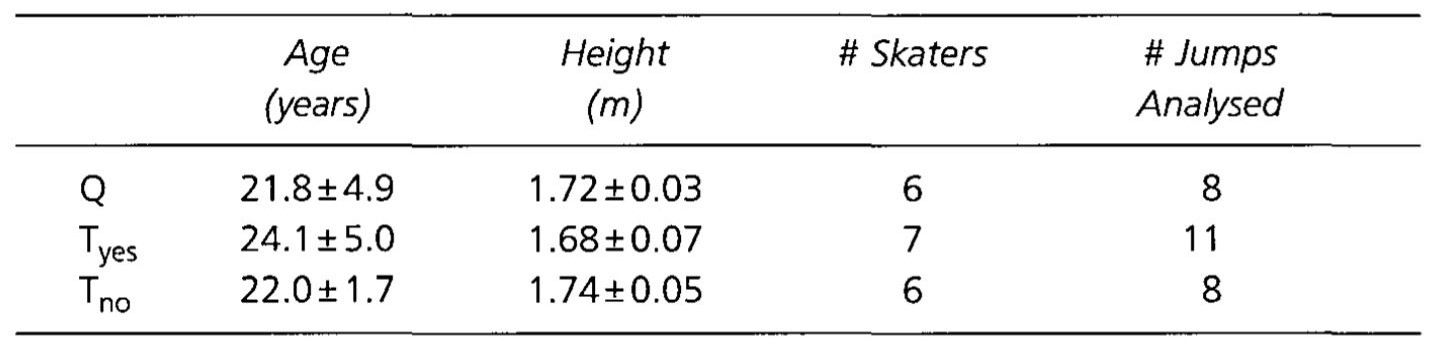
\includegraphics[width=\linewidth]{toe_ages.JPG}
	\caption{The Ages of the Skaters}
	\label{Fig:ToeLoopAges}
\end{figure}
"Four key events were identified for each jump: toe-pick (instant the toepick was placed into the ice); take-off (last contact with the ice); max height
(top of the flight phase); and landing (instant of contact with the ice).
Additionally, each jump was divided into three phases: approach; propulsion;
and flight. The approach phase began at the initiation of the three
turn entering the jump and ended at toe-pick. The propulsion phase began at
toe-pick and ended at take-off. The flight phase began at the take-off and ended at landing. In total, 21 kinematic variables describing the position and motion of the skater were calculated along with the times of the propulsive and flight phases." \cite{Toe}

"Average approach speed (AppSpeed) was calculated as the average magnitude of the horizontal velocity during the approach. Knee flexion at toe-pick
was calculated for the glide (GlideKneeTP) and take-off (TOKneeTP) legs and
reported such that zero degrees correspond to a fully extended position. For all skaters except one, who jumped the opposite direction, the glide leg was the right leg and the take-off leg was the left. Toe-pick distance (TPDist) was calculated as the horizontal distance between the heel of the glide foot and the toe of the take-off foot at the instant of toe-pick. Vertical (VelVT0) and horizontal (VelHT0) velocities at take-off were calculated for the centres of mass of the
skaters. Take-off angle (AngleT0) was calculated as the inverse tangent of the
VelVTC)
 divided by the VelHT0. Backward tilt (Tilt) was defined as the angle
between the longitudinal axis of the skater's trunks and a vertical axis that was
projected onto a vertical plane parallel to the skater's direction of travel during
the flight phase. Average rotational velocity (RotVel) was calculated from the
hip segment about the longitudinal axis during the flight phase. Maximum
jump height was defined as the maximum vertical displacement of the CM of
the skaters during flight. Hip and shoulder rotation angles (Figure 4), measured
as the angle between the two hips and shoulders, respectively, and a line perpendicular to the direction of travel of the jump in the horizontal plane, were calculated at toe-pick (HipRotTP, ShRotTP), take-off (HipRotT0, ShRotTO) and
landing (HipRotLAND, ShRotLAND). Heights of the CM at the take-off
(HeightCMT0) and at the landing (HeightCMLAND) were calculated as the vertical position of the CM above the ice surface at these two instances. Lastly, to
measure the openness or closedness of the skaters' positions, in terms of arm
and leg position, a variable, body position (BodyPos), was defined. Body position was detemined by averaging the distances of the two wrists and free (glide)
leg ankle from the longitudinal axis of the skater in the transverse plane of the
skater at take-off, throughout the flight phase, and at landing (Figure 5). This
measure was chosen in lieu of reporting the skaters' moments of inertia to provide coaches with a practical measure that is easily visualised in comparison to
the body positions that their own skaters assume during these jumps. The measure was adapted from an ankle to ankle position measure reported by Albert
and Miller (1996) in a study of double Axels. A comparison the BodyPos
variable and the moment of inertia calculated about a skater's longitudinal axis for a quadruple toe-loop is provided in Figure 6. Notice that the two variables follow a similar trend throughout the phases of the jump, but that the scale
on BodyPos has a more immediate visual meaning to the non scientist since it
is reported in metres. Variables dependent on stature, TPDist, HeightC0M, and
BodyPos, were scaled using a ratio to the skaters' heights to the average height
of the skaters."\cite{Toe}
\begin{figure*}[h]
	\centering
	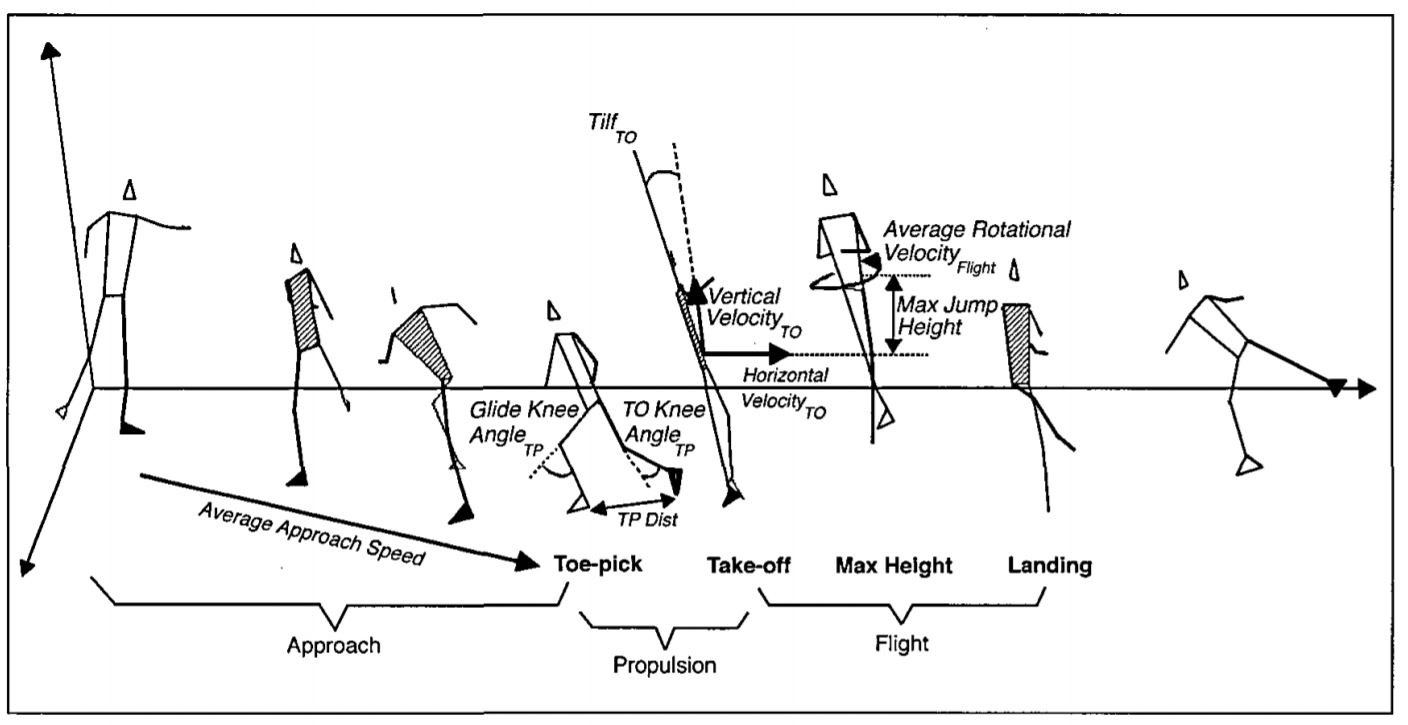
\includegraphics[width=\linewidth]{ToeLoop.JPG}
	\caption{Toe Loop Jump(Scientific)}
	\label{Fig:AxelJump}
\end{figure*}

\subsubsection{The Study Results of The Triple/Quad Toe Loop}
"The average horizontal approach speeds were similar for all jumps (Table 2)
with the Q jumps on average only 6% slower as compared to the Tyes
 jumps." \cite{Toe}
"Through the approach, as the skaters prepared for the toe-pick, there was gradual downward motion of their centres of mass due to flexion of the glide knee.
The knees of the glide legs then started to extend on average 0.12 to 0.14 s prior
to toe-pick. The toe-pick of the take-off foot was placed into the ice an average
of 0.76m from the glide foot for the Q jumps and generally centred behind the
right hip. Toe-pick distance tended to be slightly less for the Q jumps as compared to the Tyes
 jumps. However, TPDist was somewhat variable from jump
to jump for individual skaters and not all skaters who completed both quadruple and triple toe-loops consistently had shorter TPDist for their Q jumps.
Both the timing and positioning of the hip and shoulder rotation in this
phase was slightly different across groups (Table 2). The Tno group opened
their hips more during the approach so that by toe-pick the hips were rotated
on average 8 degrees farther into the jump as compared to the Tyes
 or Q groups.
Additionally, for the Tno jumps, the shoulders were lagging on average 26
degrees behind the hips at toe-pick. A similar technique was observed for the
Tyes
 jumps, for which shoulder rotation was on average 32 degrees behind hip
rotation. However, for the Q jumps, the skaters started rotation of the shoulders
earlier in the approach so that at toe-pick the shoulders were on average only 6
degrees behind the rotation of the hips." \cite{Toe}

%The Flip Jump -------------------------------------------------------------

\section{The Flip Jump}

\subsection{The Physics of The Quad Flip}
The study was conducted with the assistance of Waseda University figure skating club
(Saitama, Japan). One nationally ranked competitive male figure skater participated in the study to
perform single, double, and triple flip jumps. 

Data collection consisted of three sections: single, double, and triple flip jumps. All data were
collected simultaneously by five IMUs (product series: LPMS-B2, LP-Research, Tokyo, Japan) and six
high-resolution cameras (FDR-AX100, SONY). Five IMUs were attached to the skater with a special
uniform. Real-time sensor signals were recorded at the rate of 100 Hz by a mobile phone based on
wireless transmission. Five body segments of the skater were outfitted with IMUs on the posterior side
at the following approximately positions: the 2nd thoracic vertebra (D1), the 4th–5th lumbar vertebra
(D2), the center of mass of left thigh (D3), the center of mass of left shank (D4), and mid-sole of the left
skate boot (D5; Figure 1b). Sensor coordinate system S (X’Y’Z’) was aligned with the global coordinate
system G (XYZ) automatically based on gravity and magnetic field (Figure 1a). Six high-speed cameras
were placed around the ice rink to record video data at a frame rate of 60 fps to be used as reference.
The skater warmed up both off-ice and on-ice for a total of 20 minutes, then performed seven
single, fourteen triple, and nine double flip jumps successively. The received signals of triple jumps
included nine successful jumps (3Fo), which were trials that landed clearly on the right outside edge,
three unsuccessful jumps (3Fx), which are trials that landed with the center of mass of the body
deviating from landing leg (landed two-foot, stepped out, and fell), as well as two popped jumps
(3Fp), which are trials that performed with fewer rotations than intended (single rotation in these two
cases). All received single (1F) and double signals (2F) were classified as successful trials. 

Data processing was performed by MATLAB R2017a. In this study, kinematic parameters at
take-off event and during the flight phase were calculated from raw signals. Raw signals consisted
of three parts: angular velocity (degree/s), Euler angle (degree), and linear acceleration (g) [8]. These
signals were filtered by Butterworth low-pass filter with cut-off frequency of 10 Hz. Then linear
acceleration expressed in coordinate system S from D2, which was attached approximately to the
center of mass of the body, was transformed to be expressed in coordinate system G by using Euler
rotation matrix. Euler rotation sequence was set with the order of X’Y’Z’ in LPMS-B2. Since the indoor
environment and mobile phone signal interfered with magnetometer during coordinate system
alignment, only Z’-axis direction was precisely aligned to the vertical, upward Z-axis direction based
on gravity (Figure 1a); vertical velocity (VV), which was the value of Z-axis velocity in coordinate
system G, was acquired using rotation matrix with incomplete X’Y’ Euler rotation sequence to
transform velocity vector from coordinate system S to coordinate system G. Firstly, D2 velocity in
coordinate system S was obtained by numerically integrating D2 linear acceleration after removing
the moving average in order to minimize the integral drift. Then the transformation of velocity vector
between coordinate systems was conducted using incomplete rotation matrix: 

%where 𝑣௑ି௒ and 𝑣௒ି௑ are velocity components in two orthogonal directions in X-Y plane of
%coordinate system G; 𝑣௓ is Z-axis velocity component in coordinate system G; 
%𝑣௑ᇱ, 𝑣௒ᇱ, and 𝑣௓ᇱ are X’-axis, Y’-axis and Z’-axis velocity components in coordinate system S, respectively; 𝜃௑ᇱ, and 𝜃௒ᇱ are X’-axis and Y’-axis Euler angles, respectively. The value of 𝑣௓ was defined as VV. In this study,
%none of Y’-axis rotations of IMUs exceeding the range of −89 to 89 degrees avoided singularity problem.
The moment when vertical velocity reached maximum value was defined as take-off event (Tto), and
the moment of minimum was defined as landing event (Tland) for all trials. The time interval between
Tto and Tland was defined as flight phase. Flight time (FT) was calculated as Tland-Tto (Figure 1c).
Video data was used to obtain the time interval between take-off and landing events as the gold
standard for FT. Percent root-mean-square error (RMSE\%) between gold standard FT and FT derived
from D2 signals was computed for 1F, 2F, 3Fo, 3Fx, and 3Fp by the following formula: 
Another four kinematic parameters derived from body segments were computed to determine
the co-movement within body. These parameters are differences of angular velocity between thorax
and pelvis (DiffAV(tho-pel)), pelvis and thigh (DiffAV(pel-thi)), thigh and shank (DiffAV(thi-sha)),
as well as shank and sole (DiffAV(sha-sol)), calculated by subscribing Z-axis angular velocity
expressed in coordinate system G from two adjacent IMUs

\subsubsection{The Results}
Table 1 demonstrates an overview mean ± standard deviation for all thirteen kinematic
parameters as well as the results of F-test among 1F, 2F, and 3Fo. Nine parameters derived from the
center of mass of the body at Tto and during flight phase were observed to have significant statistical
differences among 1F, 2F, and 3Fo. VV of 1F at Tto increased dramatically by 72.7% compared with
2F on average (p < 0.0001), whereas this increment was 10.7% from 2F to 3Fo (p = 0.006). AV during
flight phase increased by 112.5% from 1F to 2F (p < 0.0001), 26.1% from 2F to 3Fo (p < 0.0001), and
168.0% from 1F to 3F (p < 0.0001). HV at Tto decreased by 35.50% from 1F to 2F (p < 0.0001) and 31.09%
from 1F to 3Fo (p < 0.0001). ToA at Tto increased by 97.62% from 1F to 2F (p < 0.0001) and 104.41%
from 1F to 3Fo (p = 0.01). ToT at Tto for 3Fo increased by 56.5% (p = 0.008), and in the case of 2F,
increased by 29.9% (p = 0.01) on average when compared with 1F. Comparing TtoTP during flight
phase, it takes the skater 0.42 s to hold his limbs close to the body to the tightest position in order to
achieve his maximum angular velocity during performing a 3Fo, which was 67.7% of FT, while this
duration was reduced by 52.4% on average in 2F (p < 0.0001), which was 37.0% of FT. Concerning 1F,
TtoTP was approximately 0.08 s on average. RinA in the case of 3Fo showed as an average of 1.84,
which was 61.3% of completed revolutions. Concerning 2F and 1F, RinA were 64.0% and 53% of
completed revolutions. When comparing four kinematic parameters derived from body parts,
DiffAV(tho-ple) and DiffAV(ple-thi) at Tto showed a significant difference between group 1F and 2F
(p = 0.02; p = 0.0005). 


%Axel Jump -----------------------------------------------------------------
\section{The Axel Jump}
"The Axel Paulsen jump (Axel or A) is the most technically
difficult jump of all figure skating jumps, which is why it is at the
top of the International Skating Union (ISU) Judging System
Code of Points (CoP). It can be divided into three phases: the
entrance phase, which ends with the take-off; the flight phase,
when the skater is rotating in the air; and the landing phase,
which starts at the exact moment when the blade touches the
ice and ends when skater is safely skating backwards on the full
outside edge with one leg behind in the air." \cite{Axel}

\subsection{The Physics of The Quad Axel}
"The research involved one Polish elite male junior skater.
He was the first one in Poland to have ever performed the triple Axel (3A), the quadruple Toe Loop (4T), or the quadruple
Salchow (4S). He was 170 cm tall and had a body mass of 68 kg.
In order to obtain kinematic data, two Canon LEGRIA HV40
(frame rate 50 Hz) cameras were positioned on the ice rink at an
angle of approximately 90 degrees in relation to each other. The
camera settings were carefully planned in order not to disturb
the usual skating trajectory of the skater (Fig. 1). Both cameras
recorded all the phases of each of the jumps (Fig. 2) in order to
achieve a 3D effect. The video cameras were turned on to record
the 1.5 x 1.5 x 2.0 m calibration frame box and were then removed from the ice rink. The cameras remained turned on for
the duration of data collection." \cite{Axel}
"The APAS 2000 program also automatically calculated the
centre of gravity of the skater (CG) and generated the kinematic
data of each jump. The parameters taken into consideration in
further analysis were: both leg joint angles ($\alpha$, $\beta$, $\delta$, $\alpha$’, $\beta$’, and $\delta$)
and the take-off angle ($\Upsilon$, $\deg$) (Fig. 4), height of flight (hmax, m)
(defined as the highest position of the skater’s centre of gravity
above the ice rink surface), and the horizontal %(υxz, m/s) 
and
vertical velocity %(υy, m/s)
of the CG.
The skater performed all the jumps entering on the left and
landing on the right leg. That is why in the analysis, during the
entrance phase (n), the left leg was the supporting leg, and the
joint angles which were analysed were $\alpha$, $\beta$,and $\delta$. During the landing phase (w), the right leg became the supporting one so angles $\alpha$’, $\beta$’, and $\delta$’ were analysed.
Besides the joint angles, the take-off angle ($\Upsilon$) (Fig. 4) was
analysed. The take-off angle can be defined as the angle between
the ice rink surface and the vertical axis of the skater’s body at
the moment of take-off."
"The most significant moments during the entrance phase
(n) are the transition zone, called also the pre-take-off phase,
and the take-off itself. The beginning of the transition zone was
operationally defined as the start of the skater’s upward motion
signified by the beginning of the positive vertical velocity of the
skater’s centre of gravity %(υy)
. The moment of take-off was determined based on the velocity of the centre of gravity %(υ3Dsc).
Directly before the take-off, %υ3Dsc 
achieves its maximum.
Therefore, the moment of take-off was designated as the moment registered in the first recording frame after the skater
reached the maximum 
%υ3Dsc. 
Once the data had been generated,
the relative error was counted for each parameter of each jump
attempt in order to check the repeatability of the performance
of the jumps. The errors of all the parameters were lower than
10\% taken as the upper limit of normal, which showed that
there were no significant differences between the kinematic parameters of jumps with the same number of rotations in the air.
In view of these results of the relative error calculations, only
one jump of each type was taken into consideration in further
analysis."
\subsubsection{The Results}
The data obtained in the study were analysed in each specified phase of the jump. The first phase considered was the entrance.
As already mentioned, in the entrance phase, the beginning
of the transition zone was operationally defined as the start of
the skater’s upward motion signified by the beginning of the
positive vertical velocity of the skater’s CG (vy). It began an average of 0.24 s before the last contact with the ice (take-off) for 1A
and 0.22 s before this moment for 2A and 3A. Although there
were differences in the time of the pre-take-off phase between
the single Axel and the multiple rotation Axels (2A and 3A),
they cannot be considered significant.
The more rotations the skater was supposed to perform, the
lower the vertical velocity he gained was. The skater achieved
the highest horizontal velocity, of 5.42 m/s, entering the 1A; the
%υxz
 max for 2A was over 3\% lower (5.23 m/s), and that for 3A was
almost 11\% lower (4.83 m/s). Nevertheless, the biggest difference between maximal and take-off velocity (%υxz 
difference) was
observed in 3A (Tab. 1). During the 3A entrance, the skater reduced his horizontal velocity from 4.83 m/s to 2.89 m/s at the moment of take-off (40\% difference). For 2A, the reduction was
35\%, and it was 26\% for 1A.
The skater gained the highest vertical velocity of the takeoff performing 3A (3.7 m/s), and he had the lowest %υy 
in 1A
(3.19 m/s) (which means that there was a 14\% difference). The
observed differences between the %υy 
values of 2A and 3A were
very small. Moreover, the value of the take-off angle (Fig. 6) for
3A was the highest (52$\deg$), which means that the skater took off
more vertically in the triple Axel than in the other Axels. The
difference between the values of the take-off angle for 1A and 2A
was over 21\%, and it was over 36\% for 1A and 3A, both of which
were significant differences. These differences were also noticeable on the stick figures generated in the APAS program. The
skater took off much more vertically in multiple rotation jumps
(2A and 3A)" \cite{Axel}

\begin{figure*}[h]
	\centering
	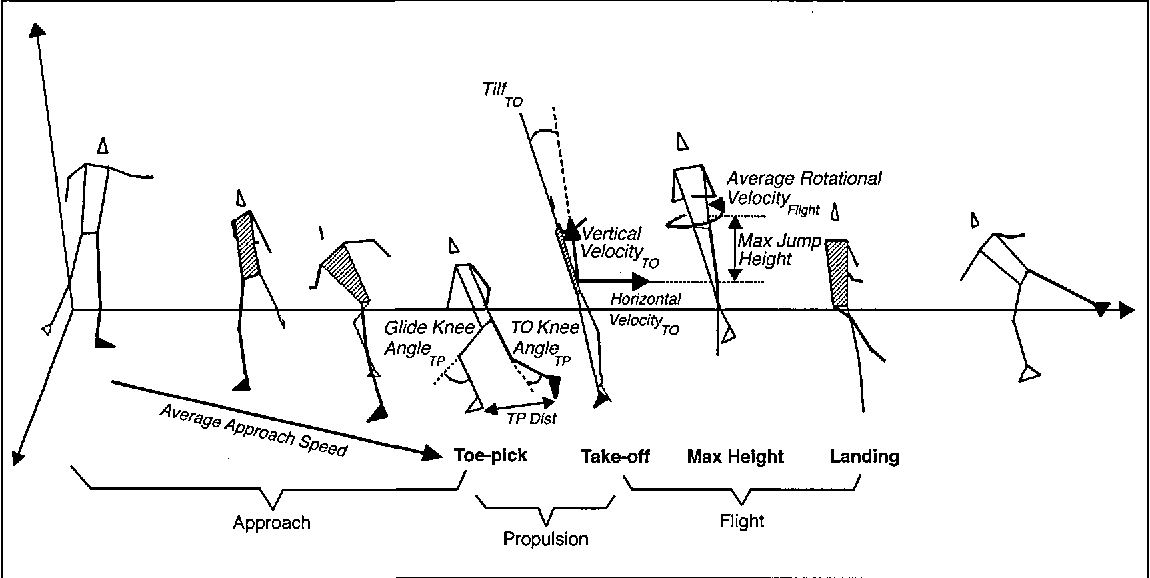
\includegraphics[width=\linewidth]{Axel_Jump.PNG}
	\caption{Axel Jump(Scientific)}
	\label{Fig:AxelJump}
\end{figure*}

%Injuries -----------------------------------------------------------------
\section{The Future}
The future of figure skating is pushing towards more intense jumps, like quad jumps. And with more intense jumps, comes the high risks of injuries. This push for more dangerous and intense jumps will make it difficult for coaches to teach the new generation of skaters and skaters will have to depend more on biomechanics to analysis their jumps. 

%Conclusion -----------------------------------------------------------------
\section{Conclusion}
This paper was about the physics of three figure skating jumps, the Toe Loop, the Flip, and The Axel. These jumps are difficult in their own right as with triple and quad versions of these jumps, the more intense, the forces are acting the skater's body. The forces acting can make a landing of a jump more difficult as landing is a way to counteract and deal with the forces at hand. 

%ACKNOWLEDGEMENT SECTION ----------------------------------------------------- 
\section*{Acknowledgements}
Thank you to the UCSC library staff and database for helping me find my resources. Thank you to Processor Gerald Moulds for assigning this and giving me an opportunity to learn. 

%BIBLIOGRAPHY ----------------------------------------------------------------

\begin{thebibliography}{1}

\bibitem{Toe}
King, Deborah et al. “Characteristics of Triple and Quadruple Toe-Loops Performed During the Salt Lake City 2002 Winter Olympics.” Sports biomechanics 3.1 (2004): 109–123. Web.

\bibitem{Sal}
Cristian Romagnoli et al. “2D Video Analysis System to Analyze the Performance Model of Figure Roller Skating: A Pilot Study.” Proceedings 49.155 (2020): n. pag. Web. 

\bibitem{Axel}
Mazurkiewicz Anna, Iwańska Dagmara, and Urbanik Czesław. “Biomechanics of the Axel Paulsen Figure Skating Jump.” Polish journal of sport and tourism 25.2 (2018): 3–9. Web.

\bibitem{Flip}
Yuchen Shi, Atsushi Ozaki, and Masaaki Honda. “Kinematic Analysis of Figure Skating Jump by Using Wearable Inertial Measurement Units.” Proceedings 49.124 (2020): n. pag. Web.



\end{thebibliography}

%Optional: BIOGRAPHY Section -------------------------------------------------
 
% If you have an EPS/PDF photo (graphicx package needed) extra braces are
% needed around the contents of the optional argument to biography to prevent
% the LaTeX parser from getting confused when it sees the complicated
% \includegraphics command within an optional argument. (You could create
% your own custom macro containing the \includegraphics command to make things
% simpler here.)
%\begin{biography}[{\includegraphics[width=1in,height=1.25in,clip,keepaspectratio]{mshell}}]{Gerald Moulds}
% or if you just want to reserve a space for a photo:
\begin{IEEEbiography}
    [{
\includegraphics[width=1in,height=1.25in,clip,keepaspectratio,angle=90]{Bio.JPG}}]{Christy Yuen}
I am a University of California, Santa Cruz student. I am a Computer Science senior student. I grew watching the Olympics and found figure skating and the physics of it, fascinating. I am no means an expert on this topic, I found resources that help me understand and deepen my interest in the physics of figure skating. 
\end{IEEEbiography}

%\vfill

% Can be used to pull up biographies so that the bottom of the last one
% is flush with the other column.
%\enlargethispage{-5in}

\end{document}
